\section{Backend}

\subsection{Využité technologie}
Jako stavební kámen pro backendovou část byl použit Node.js s frameworkem Express.js. Na samotném Expressu běží GraphQL, které se stará o dotazy. Dále je zde také zaregistrován zpracovatel dotazů pro GraphQL Subscription který zodpovídá za komunikaci v reálném čase.\par
Při použití jednoho serveru by bylo možné provozovat GraphQL Subscription pouze pomocí paměti. Pokud bychom však chtěli rozdělit zátěž mezi více serverů tak by nám ne vždy došel dotaz pro poslouchajícího klienta (například: Klient si vytvořil komunikaci mezi sebou a serverem číslo 1. Další dotaz z jiného zařízení přišel na server 2, server tomuto zařízení odpověděl zpět bez problému, ale nebyl schopen dát vědět zařízení číslo 1 o tom, že se něco stalo, protože tyto 2 servery o sobě navzájem neví). Proto je potřeba využít funkci Redisu s názvem Pub/Sub\cite{PubSub} díky které se dá vědět všem serverům při dotazu.\par
Jako databáze byla zvolena databáze MongoDB, kvůli možnosti zpracovávat velké množství dat. Pro propojení backendu a databáze byla použita Prisma. Na dotazy, které by se často opakovaly, by nebylo exektivní se stále dokola dotazovat databáze, proto se určité, často opakované dotazy ukládají do cache paměti Redis.\par

\subsection{Autorizace}
Pro přístup k většině dotazů je potřeba být přihlášen. Uživatelé se můžou registrovat pomocí mutace "register" a přihlašovat pomocí "login". Při registraci jsou uživateli zkontrolovány vstupní data, je vytvořen dokument v těmito hodnotami (heslo je zahashováno pomocí bcrypt\cite{bcrypt}), vytvořena session a následně vrácen hash s ukrytým ID této session a jménem uživatele. Přihlášení potom funguje velmi podobně jako registrace, ale místo vytváření nového uživatele se hledá uživatel se stejným emailem a kontroluje se jestli přiložené heslo sedí s tím v databázi.\par
K přístupu k dotazům, ke kterým je potřeba být přihlášen, je potřeba zaslat v hlavičce dotazu vlastnost s názvem "authorization" s hodnotou "Bearer TOKEN".\par
Pokud se chce uživatel odhlásit tak by měl zavolat na mutaci "logout", která smaže aktuální session z databáze aby se s ním nebylo možné dálé hlásit.\par
Při ztrátě hesla je pak možné zavolat na mutaci "sendResetPassword" s parametrem email. Pokud na zadaném emailu existuje účet tak je na něj zaslán email s odkazem obsahující resetovací token. Pomocí mutace "resetPassword" je při přiložení tohoto tokenu do 10 minut možné heslo změnit.\par
%//TODO Vysvětlit token?
Kvůli bezpečnosti je také nutné mít možnost uživatelský účet smazat. Pro tento účet slouží mutace "deleteAccount", při které musí být uživatel přihlášen a musí zadat aktuální heslo. Při této akci se nenávratně mažou všechna uživatelská data.

\subsection{Ovládání hry}
Jako jádro pro komunikaci mezi telefonem a hrou slouží subscription s názvem "unityCommunication". To potřebuje jako argument token s přihlášením, protože při navazování WebSocketu se nezasílá hlavička dotazu.\par
Pro získání ostrovů a úrovní slouží query "islands" a "levels". Obě tyto query obsahují číslo ostrovu/levelu, data pro samotnou hru nebo mobilní telefon a úroveň obsahuje navíc počet hvězd, pokud již hráč tento level hrál.\par
Pro nastavení aktuálního ostrova nebo úrovně se používají mutace "setUnityIsland" a "setUnityLevel". Obě nic nevrací a slouží k zasílání příkazů pro hru v prohlížeči.\par
Když hra potřebuje načíst ostrovy je potřeba zavolat na mutaci "getUnityIslands". Tato mutace nic nevrátí, ale ihned posílá hráči pomocí subscriptiony data pro vykreslení.\par
Pro nastavení rycholosti přehrávání výsledné animace slouží mutace "setSpeed", pomocí které se dá nastavit rychlost v rozmezí mezi 1x až 10x.

\subsection{Přihlášení pomocí QR kódu}
Aby uživatel nemusel psát heslo na chytré televizi nebo na zařízení bez klávesnice, je možné se přihlásit pomocí QR kódu. První se musí zaregistrovat k odposlouchávání zařízení na kterém se chce uživatel přihlásit pomocí subscription s názvem "qrLogin". To bere jako argument text, který je pak hodnota pro přihlášení se. Potom lze z již přihlášeného zařízení zavolat na mutaci "qrLogin" s stejným argumentem jako u subscription.

\subsection{Vyhodnocování úrovně}
Ještě před ukázáním zádání je potřeba zažádat server o čas začátku řešení, aby bylo možné na konci zjistit jak dlouho hráči trvalo vyžešit úroveň.\par
Samotné vyhodnocování úrovní probíhá v několika krocích viz obrázek \ref{fig:proces-vyhodnocovani}. Tyto kroky jsou rozepsané v následujících podkapitolách.

\begin{figure}[h]
    \centering
    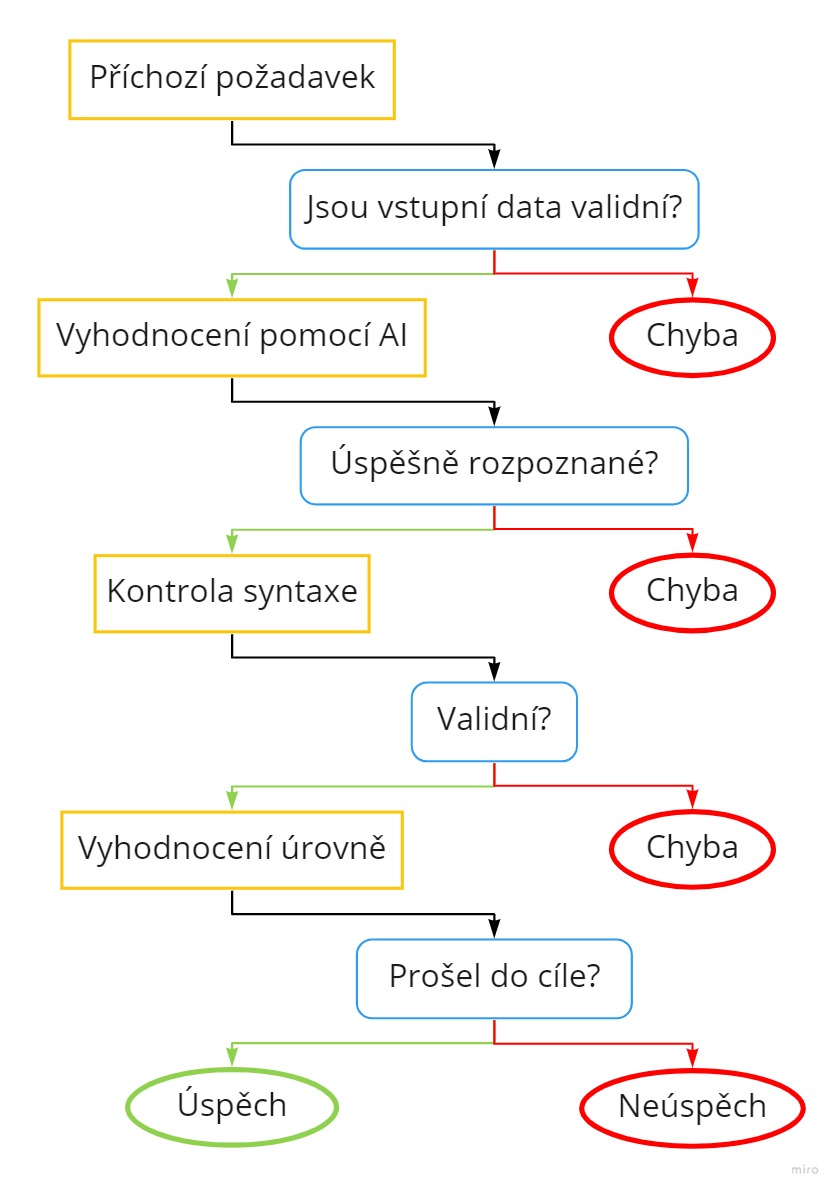
\includegraphics[width=0.3\textwidth]{img/proces.jpg}
    \caption{Proces vyhodnocování úrovně.}
    \label{fig:proces-vyhodnocovani}
\end{figure}

\subsubsection{Validace vstupů}
\subsubsection{Vyhodnocení pomocí AI}
\subsubsection{Kontrola syntaxe a vyhodnocení úrovně}